

\chapter{Installation and Commissioning}
\label{ch:install}

\section{Introduction}

This chapter discusses the LAr-FD Installation and Commissioning system's activities and responsibilities.  
LAr-FD construction and installation will occur in a series of distinct phases:

\begin{itemize}
\item installation planning and prototyping
\item surface storage identification and operation
\item excavation and outfitting of the cavern; this activity is the responsibility of the Conventional Facilities subproject (CF), 
\item construction and installation of the cryogenics system and cryostats by a construction management firm; this activity is the responsibility of the cryogenics system 
\item construction of LAr-FD components at collaborating institutions and shipment to the Far Site
\item installation of detector components and installation management
\item commissioning activities leading to CD-4
\end{itemize}

The Installation and Commissioning system will accept responsibility for the LAr-FD cavern, associated tunnels, infrastructure and above-ground facilities from Conventional Facilities upon completion of the Conventional Facilities contract. The cavern will be outfitted with the following utilities upon receipt of beneficial occupancy:

\begin{itemize}
\item ventilation in accordance with OSHA standards
\item electrical power sufficient for the HVAC, cryogenics plant cooling and general 110-V service
\item quiet power for the electonics with a double Faraday-shielded transformer located some distance from the cavern to take advantage of the inductance of the power lines. The primary shield will be connected to the main substation via a grounded feed wire and the secondary shield will be connected to the Ufer ground.
\item communications consisting of telephone lines and computer network
\item cavern lighting in accordance with OSHA regulations for industrial use
\item tunnel lighting with battery-powered backup or emergency circuit backup
\item environmental monitoring of oxygen, carbon monoxide, smoke and temperature
\item dual isolation bulkheads separating the cavern from the existing Far-Site facility
\item sump pumps for groundwater removal
\end{itemize}

After beneficial occupancy of the completed cavern from the 
CF subproject, the cavern ventilation system will be tested to assure adequate performance with regard to ODH requirements. The system will be tested with oxygen monitors distributed around the cavern and a controlled argon spill. Remedial action will be taken if required during cryostat and cryogenics construction.

The cryostat and cryogenics contractor will retain responsibility for the site during construction of the cryostat and cryogenics system. The Cryostat and Cryogenics System group will provide oversight during this phase. Upon completion of this contract, the facility will be in the following state:

\begin{itemize}
\item the LN2 refrigeration system will be constructed and commissioned with liquid nitrogen
\item the LAr systems and cryostats will be constructed and tested without the introduction of cryogens \item the access hatches on the cryostat and the cryostat feedthroughs will be temporarily sealed
\item the APA- and CPA-installation support beams will be in place
\item the cryostat will be connected to the steel roof structure thus connecting the detector ground to the Ufer ground
\end{itemize}

The detector will utilize the cryostat pit rock bolts as part of the grounding scheme. The rock bolts in the pit will extend through the shotcrete that lines the cavern and be attached to the reinforcing steel network within the cryostat concrete liner, forming an Ufer ground. The reinforcing steel will be connected to the steel truss cover. The Ufer ground will be connected to the detector ground (the cryostat SS liner) through a low-impedance connection.

The Installation and Commissioning group will be responsible for all LAr-FD-related activities at the Far Site from this point in time until the end of the LAr-FD project. Close coordination is clearly required between this group, system groups that provide components and other Far Site construction activities. 

On-project commissioning activities include the coordination of system-checkout activities, culminating in the approval to introduce LAr into the detector modules, and managing the steps required to meet the CD-4 goals. 

\begin{figure}[htpb]
\centering
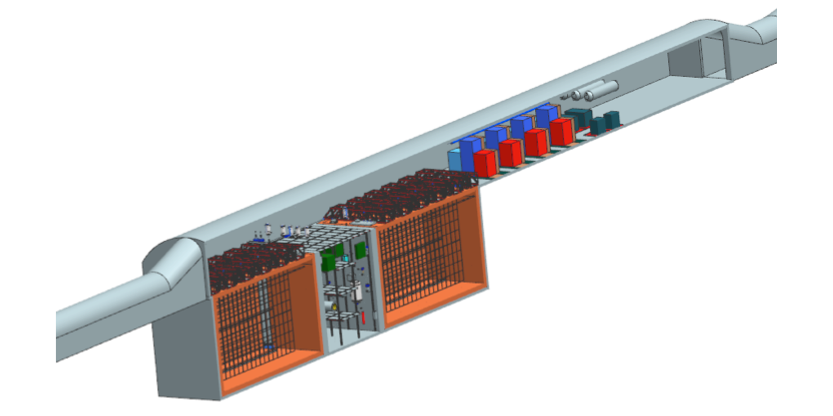
\includegraphics[width=\textwidth]{larfd-from-2794-slide9.png}
\caption{Cutaway view of two cryostats with TPC detectors installed}
\label{fig:tpc-in-two-cryostats}
\end{figure}

%%%%%%%%%%%%%%%%%%%%%%%%%%%%%%%%%%%%%%%%%%%%%%
\section{Above-ground Pre-Installation}


\begin{editornote}
  Editor's Note:  The number of shipping containers listed in this section may not be accurate as of January 2015.
\end{editornote}


Detector components will be delivered to the Far Site over a period of many months and will need to be stored in a surface-storage facility. This will allow the supply of material to be maintained ready for installation.  A facility for this purpose 
will be identified and an agreement will be made for its use during LAr-FD construction. 

The initial surface-storage plan actually includes three facilities:  a 4,000 ft$^2$ warehouse structure for material receiving and unpacking, an on-site hardstand for storage of a small number of cargo containers and an off-site hardstand area for the storage of 
a larger number of cargo containers. Material will be transferred from these areas to the cavern for installation, as required. Each system group is  
responsible for delivery of  
its components to the local storage at the Far Site or to the off-site location.  
The Installation and Commissioning group will provide the management and labor resources for inventory control, material handling and transport from the off-site and on-site storage facilities to the cavern.

\subsection{Cryostat Materials}
The on-site warehouse storage space  will initially be made available to the cryogenics system contractor who will construct the cryostats. The cryostat insulation will comprise the largest bulk of material; approximately 2,500~m$^3$. Figure~\ref{fig:gtt_storage} shows membrane-cryostat components staged in the hull of an LNG tanker under construction. 
\begin{figure}[htpb]
\centering
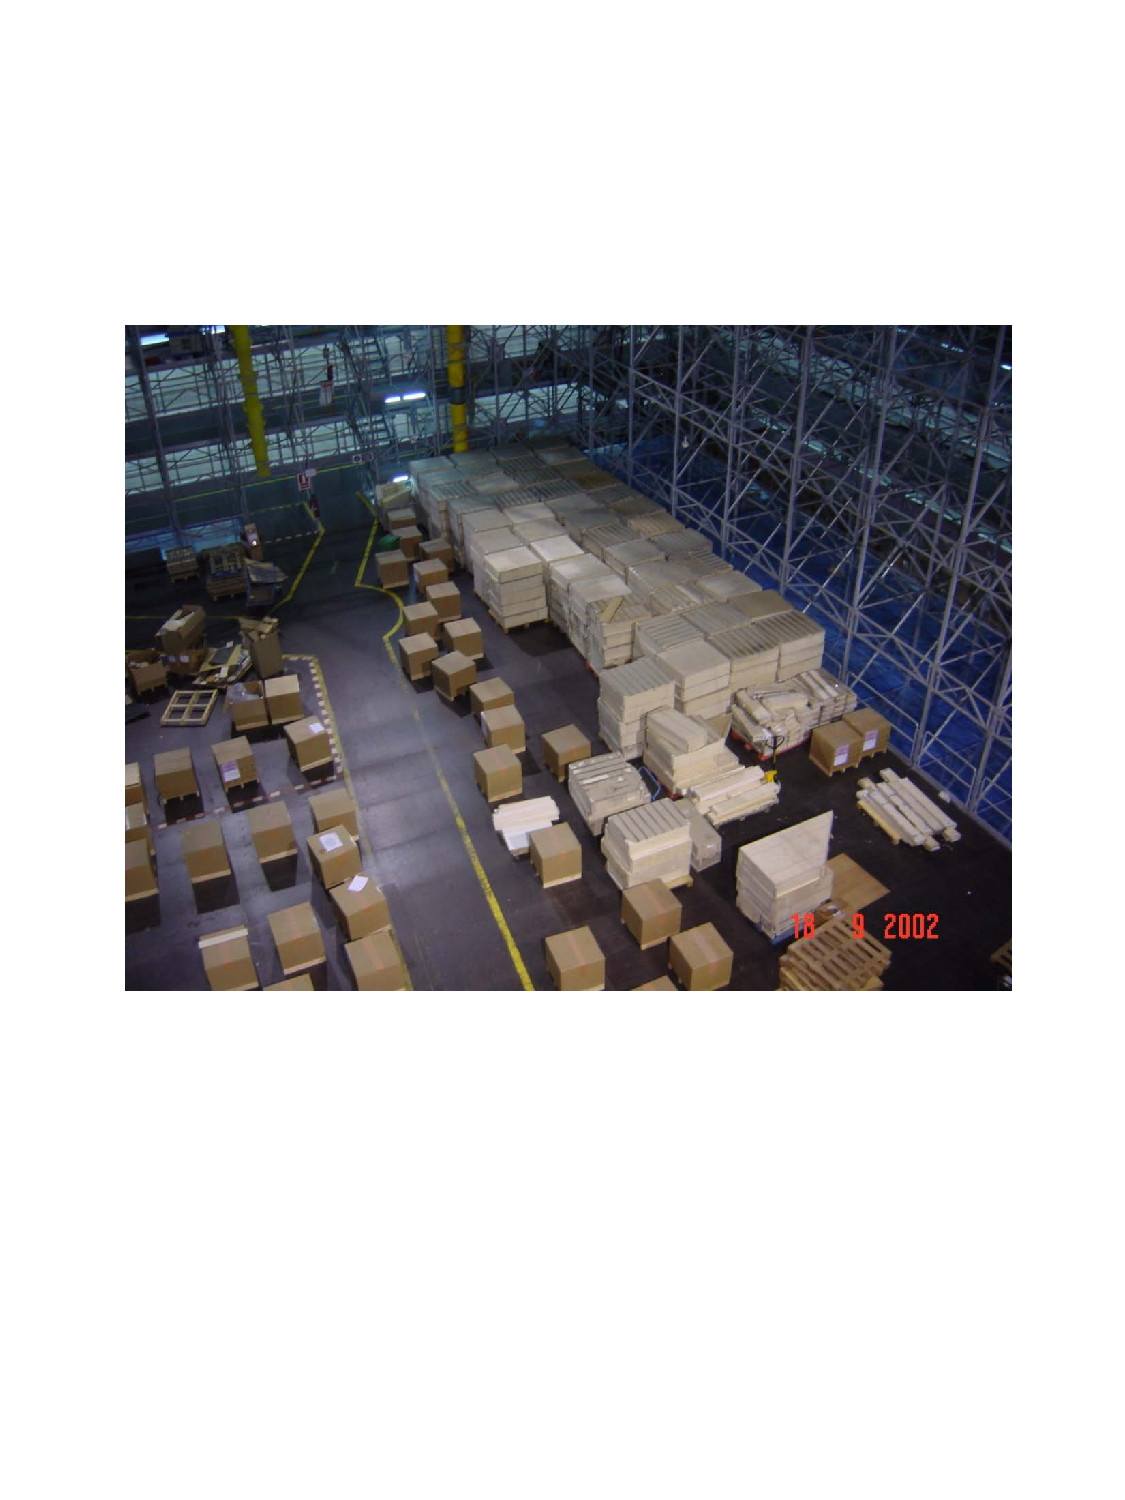
\includegraphics[width=\textwidth]{v5chIC_gtt_storage}
\caption[Cryostat components staged in a LNG transport ship]{Membrane cryostat components staged in a LNG transport ship under construction.}
\label{fig:gtt_storage}
\end{figure}
Cryostat materials will come from overseas in approximately 100 shipping containers that will be stored off-site. The containers will be brought to the shaft headframe building for unloading and transportation down the shaft.

Control of the storage area will revert to the Installation and Commissioning group when the cryostat-construction contract is completed.

\subsection{TPC Materials}

APAs and CPAs, referred to as ``TPC panels'' in this chapter, will be constructed  before arrival at the Far Site. The electronics will already be installed and the cold-testing performed. They will be shipped in sealed shipping containers to either the on- or off-site hardstand area, depending on the TPC production rate. No significant preparation or extensive testing of these components is required after arrival and prior to installation. The entire set of TPC panels for the two-cryostat detector will require approximately  fifty shipping containers. Figure~\ref{fig:apa_ship} shows a group of TPC panels in a shipping container.


Whereas general material will be lowered in a lift cage, the TPC panels are too long to fit in the lift cage and require special containers and special handling. The TPC panels, grouped in their enclosed, special containers, will be lowered down the Yates shaft since its lift has provisions to attach long objects to the bottom of the cage.
They will descend the shaft in a vertical orientation (the same orientation as they will be installed), be rotated to a horizontal orientation, then moved along the access drift  on a cart or rail to the cavern.
Figure~\ref{fig:install-yates} shows a TPC container exiting at the bottom of the shaft.  The 
TPC panels may be transported to the Far Site in these special containers or transfered to them after arrival.

TPC-panel containers will be transported to the cavern and unloaded every few days to supply the TPC components for installation. These containers may need to be moved during off-work hours to avoid conflicts with other users of the shaft lifts. TPC-panel containers may be stored in the cavern on the deck on top of the cryostat trusses. Enough parts will be stored in the cavern to ensure that a sufficient supply of TPC parts is always on hand for installation.



\begin{figure}[htbp]
\centering
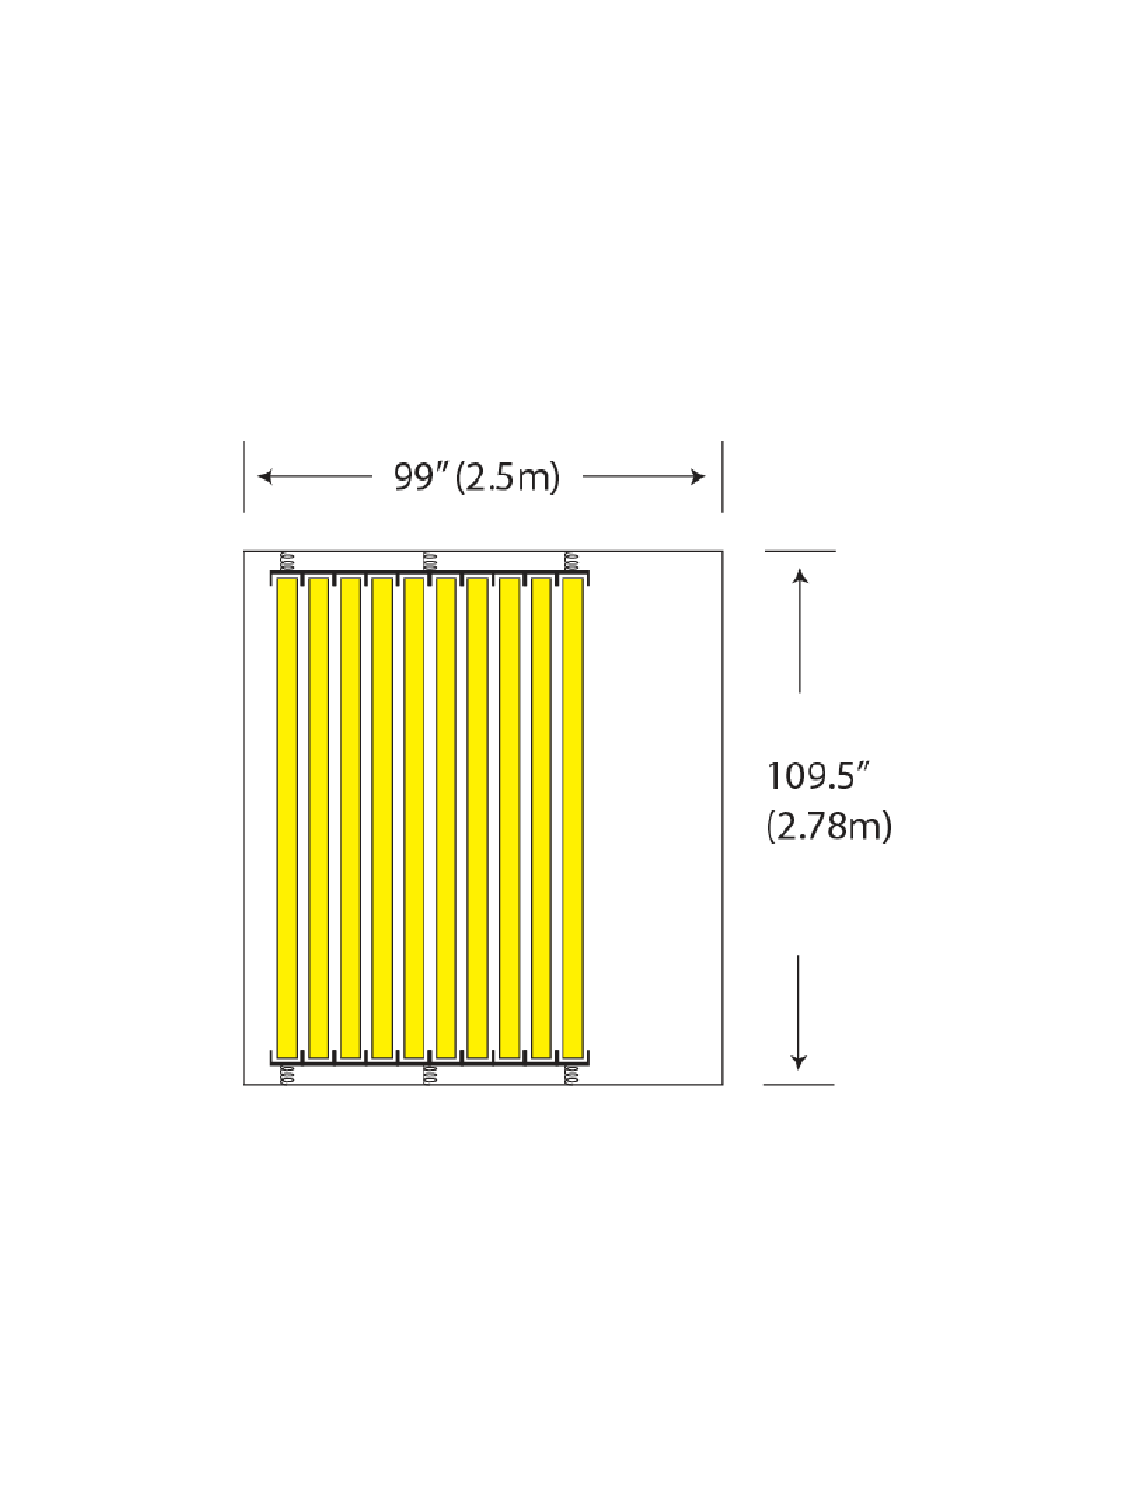
\includegraphics[width=\textwidth]{v5chIC_apa_ship}
\caption{Concept for APA shipping containers - cross section view}
\label{fig:apa_ship}
\end{figure}

\begin{figure}[htpb]
\centering
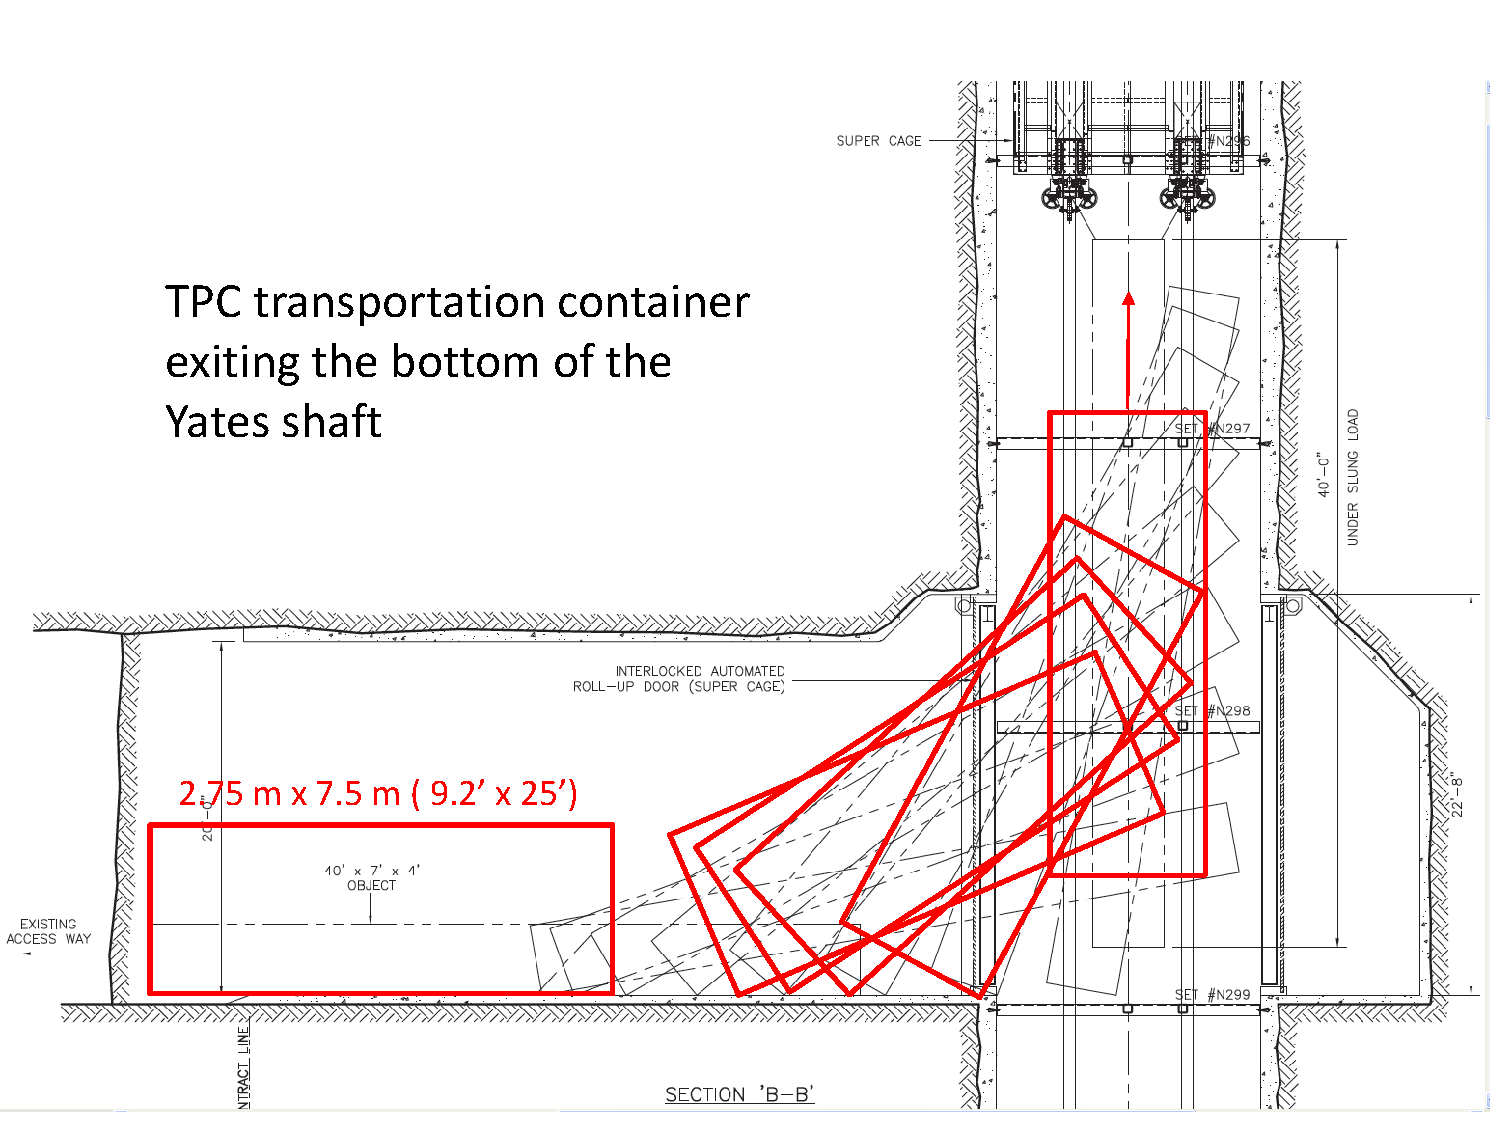
\includegraphics[width=\textwidth]{v5chIC_Yates_exit}
\caption{TPC-panel containers exiting the Yates shaft}
\label{fig:install-yates}
\end{figure}

\subsection{Liquid Argon Receipt}

Delivery of LAr will occur over a one-year period for each cryostat, with approximately six tank trucks arriving on site per day. Each tank truck will have been loaded with 18.8~tons of LAr  which will be purity-tested by the vendor before the truck departs. Minor losses of LAr will occur during shipment. The purity will be checked again during unloading. If the impurities are found to exceed the required specification, the partially emptied tank truck will be returned to the vendor.

LAr will be transferred to a buffer-storage vessel that allows the tank truck to unload as quickly as possible. Under normal circumstances transfer of the LAr out of each tank truck will require 1 hour, including the time for making hose connections and purging the hoses. The storage vessel will deliver argon to the filtering loop that processes argon from the cryostat recirculation and condensing loops.

%%%%%%%%%%%%%%%%%%%%%%%%%%%%%%%%%%%%%%%%%%%%%%

\section{Below-ground Pre-Installation}

The below-ground pre-installation activities  
must be completed prior to the start of TPC installation into the cryostat. These activities include design, procurement and installation of detector-specific infrastructure such as man-lifts, lifting fixtures, catwalks, ladders, tools, and so on. The major items include the support rails for the TPC panels, the lower staging platform for joining two panels, installation monorails for moving the panels inside and outside of the cryostat, and a mobile scaffold for providing access to the top and middle of stacked  
TPC panels.

\subsection{Equipment Required for Detector Installation}

Several items will be installed for use during TPC installation, and removed afterwards.
\begin{itemize}
\item A temporary lighting system inside the cryostat with emergency backup lighting for TPC installation
\item A ventilation system and air-monitoring sensors with alarms connected to the cryostat to assure adequate air quality for the personnel working inside the cryostat. The system will also include a high-sensitivity smoke-detection system that is interlocked to the power for all devices inside the cryostat. 
\item A raised-panel floor to protect the cryostat floor; see Figure~\ref{fig:raised_floor}. The raised-panel floor will have support spacers located between the convolutions in the stainless-steel primary membrane to provide  a flat surface for moving equipment around within the cryostat. The pressure limit for the insulation in the floor is 0.5~MPa and the load of the vacuum that will be used to monitor 
leakage during installation reduces the effective limit to 0.4 MPa.  The stock round spacers in the raised-panel floor are 10-cm diameter and would support a load of  310~kg. The load can be increased by adding larger-diameter plates under the standard spacers.
\item A transfer rail with motorized trolleys to move TPC 
panels within the cryostat
\end{itemize}

\begin{figure}[htbp]
\centering
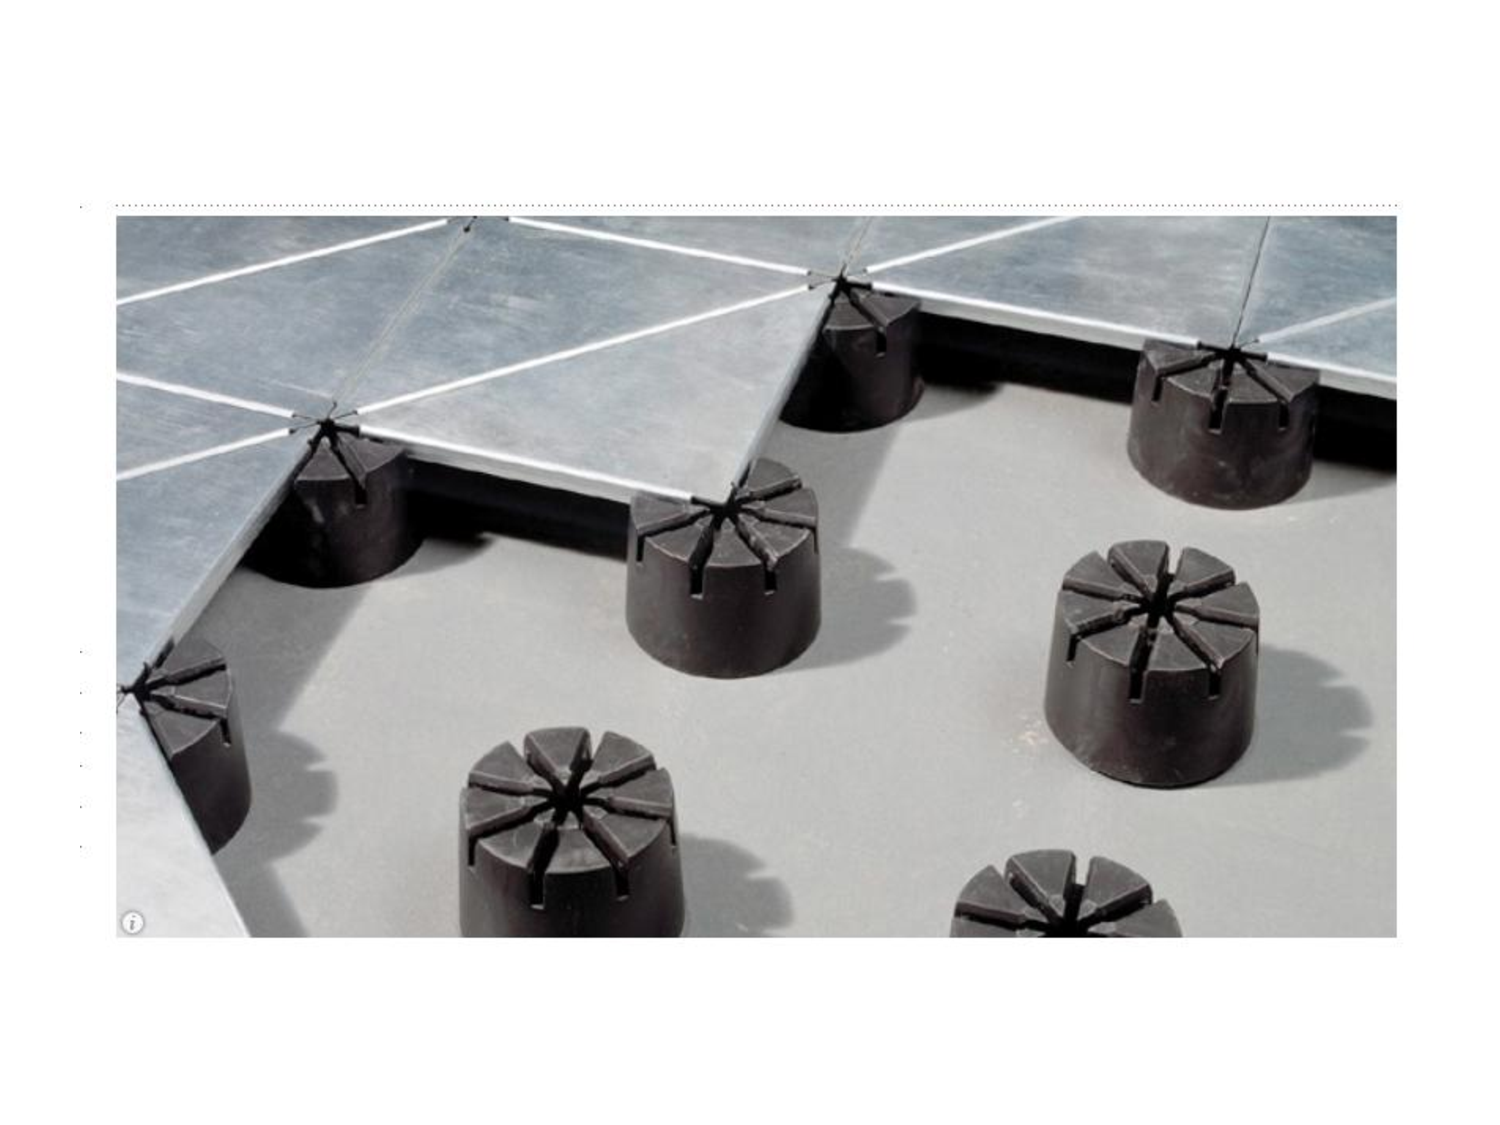
\includegraphics[width=\textwidth]{v5chIC_raised_floor}
\caption{Raised-panel floor to protect the cryostat's primary membrane }
\label{fig:raised_floor}
\end{figure}

\subsection{Clean Area}
A clean-area vestibule in the range of class 10,000 (ISO 7 equivalent) will be constructed in the septum area around the entrance to the cryostat to keep the area around the open hatch isolated from the drift access. The vestibule will have an area for personnel to gown with the appropriate clean-room clothing and safety shoes. A large, closable door, next to which the TPC-storage containers can be parked, will allow unloading of the TPC components directly from the container into the vestibule. 

A crane that operates inside the clean-room vestibule enclosure will be used to transfer 
TPC panels from the vestibule into the cryostat. The crane will have a clean-room-style hoist and trolley to prevent contamination of the cryostat or vestibule area. 

The Double Chooz detector developed a cleanliness plan to ensure that dust contamination did not contribute more than a specified amount to the detector signal. Measurements were made of the activity of rock in the underground laboratory which was assumed to be the source of airborne dust. Maximum allowable dust concentrations  
and the clean-room class and cleanliness practices were determined such as to meet the requirements for contamination. The cavern for LAr-FD and many of the access tunnels will involve new excavation with shotcrete 
covering the native rock.  
The Installation and Commissioning group will need to evaluate the dust sources in the 
LAr-FD cavern and determine if a similar approach to setting the clean room requirements is appropriate.


\subsection{Rails for TPC-Panel 
Support and Transfer}

A set of five support rails, shown in Figures~\ref{fig:work-zones} and~\ref{fig:support-rails}, permanently mounted  in each cryostat, will provide the support for the APA and CPA panels and a track for moving the panels into position. Rods spaced at 5-m intervals will support the rails. The rods will be hung from anchor points mounted in the top of the cryostat.  The rods will be adjustable to enable level installation of the rails, 
which will be done in rail segments with the aid of a laser level.
The rails shrink approximately 7~cm along their entire length during cool-down. The rods will be installed with an angle bias that allows the rails to return to level after the cryostat and TPC is cooled.

The mass of each stacked set of APA panels is 600~kg and the mass of each stacked set of CPA panels is 250~kg. The load of the TPC on the support rails comes to 200 kg/m for the APA rails and 100 kg/m for the CPA rails. The rail segments will be constructed from 20-cm-deep laser-welded, W-shaped, stainless-steel beams. The rail segments will be joined end-to-end with large pin connections. The upper support rods will be made from 15-mm-diameter stainless steel.

The rail installation can be completed most efficiently while the large scaffolding system used for cryostat construction is still in place, therefore it will be part of the cryostat-construction contract. 

\begin{figure}[htbp]
\centering
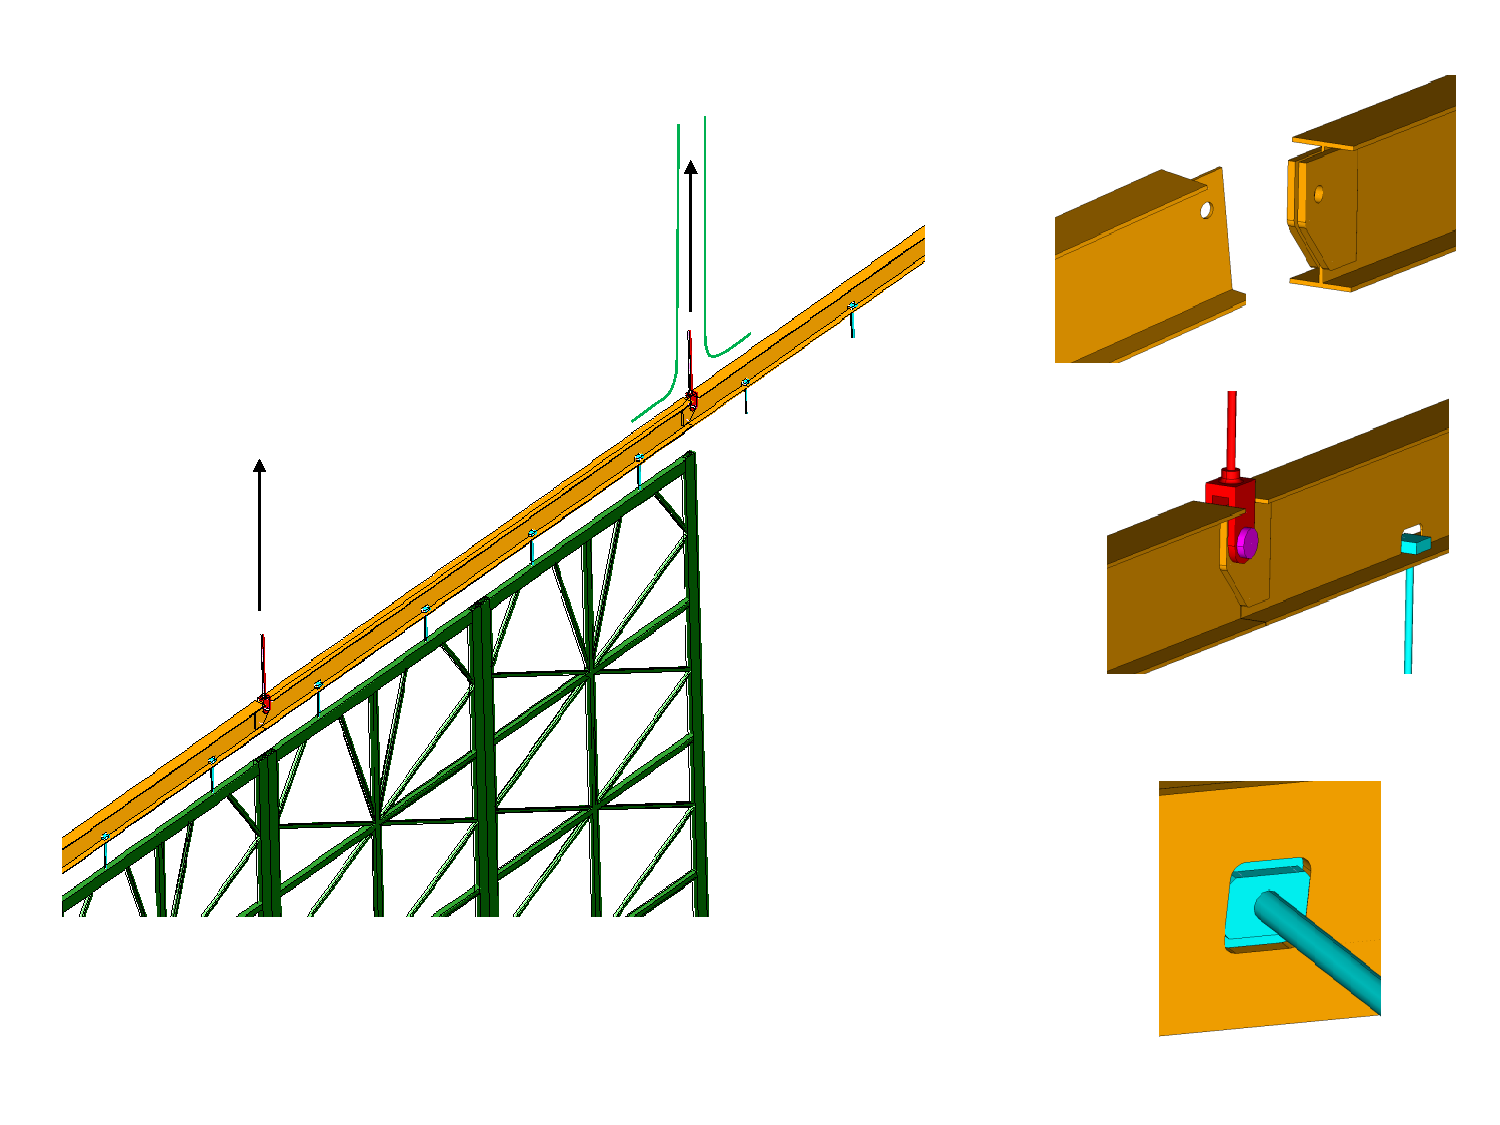
\includegraphics[width=\textwidth]{v5chIC_support-rails}
\caption{Support rails inside cryostat} 
\label{fig:support-rails}
\end{figure}

Signal and power cables will be installed from the cryostat feedthrough ports next to the APA support rods, shown in Figure~\ref{fig:feedthroughs}, along the rails to the point where the connection to the APAs will be made. The cables will be preplaced and tested before APA installation begins. 
\begin{editornote}
Editor's Note: Figure~\ref{fig:feedthroughs} is for a 17-kton fiducial mass cryostat. The 5-kton cryostat is
shorter and has fewer rows.
\end{editornote}




\begin{figure}[htbp]
\centering
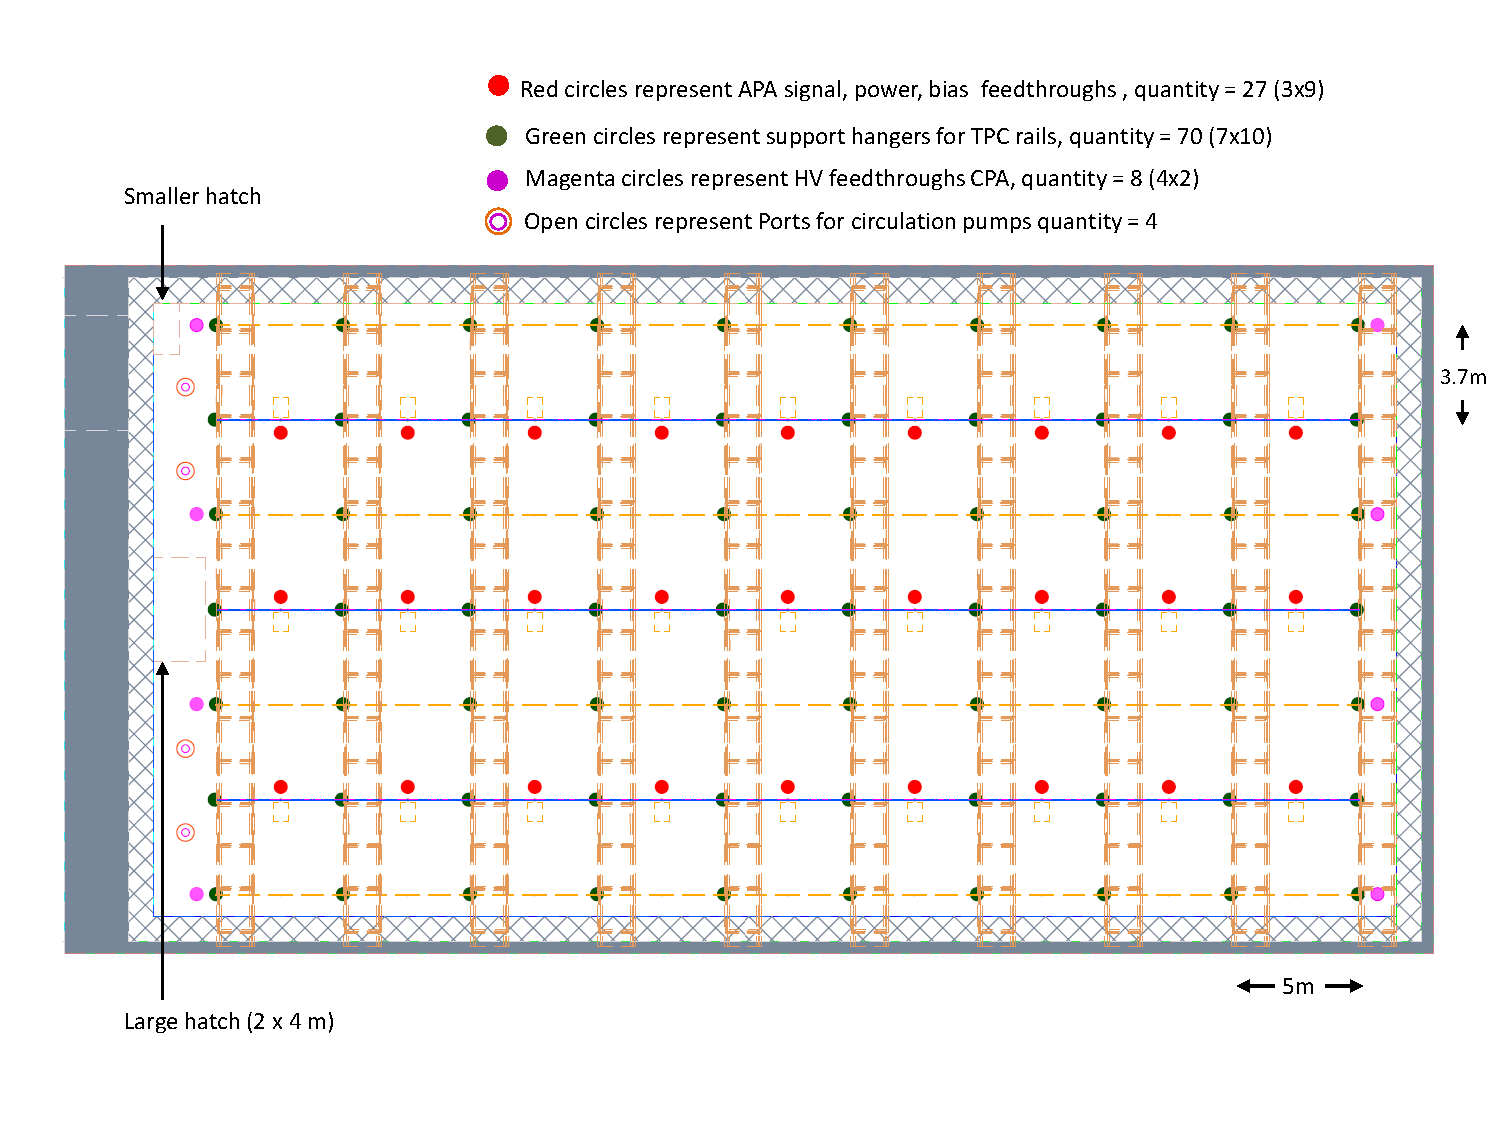
\includegraphics[width=\textwidth]{v5chIC_feedthroughs}
\caption{Feedthroughs }
\label{fig:feedthroughs}
\end{figure}

The top and bottom TPC panels of a stacked pair will be moved into the cryostat separately, then connected together below the cryostat equipment hatch. The lower panel is held temporarily with a staging platform while the upper panel is connected.  After connection, a motorized trolley will move the stacked panels from the hatch area to the final position. Since the duty cycle of the trolley is rather low, the trolley could be battery-powered to avoid the need for cable festooning. The trolley initially moves along a transfer rail until it reaches the end where the stacked panel will be permanently mounted. An arrangement of transfer switches is used to connect the transfer rail to the final support rail. See Figure~\ref{fig:installation-monorail} for an example of a transfer rail.


\begin{figure}[htpb]
\centering
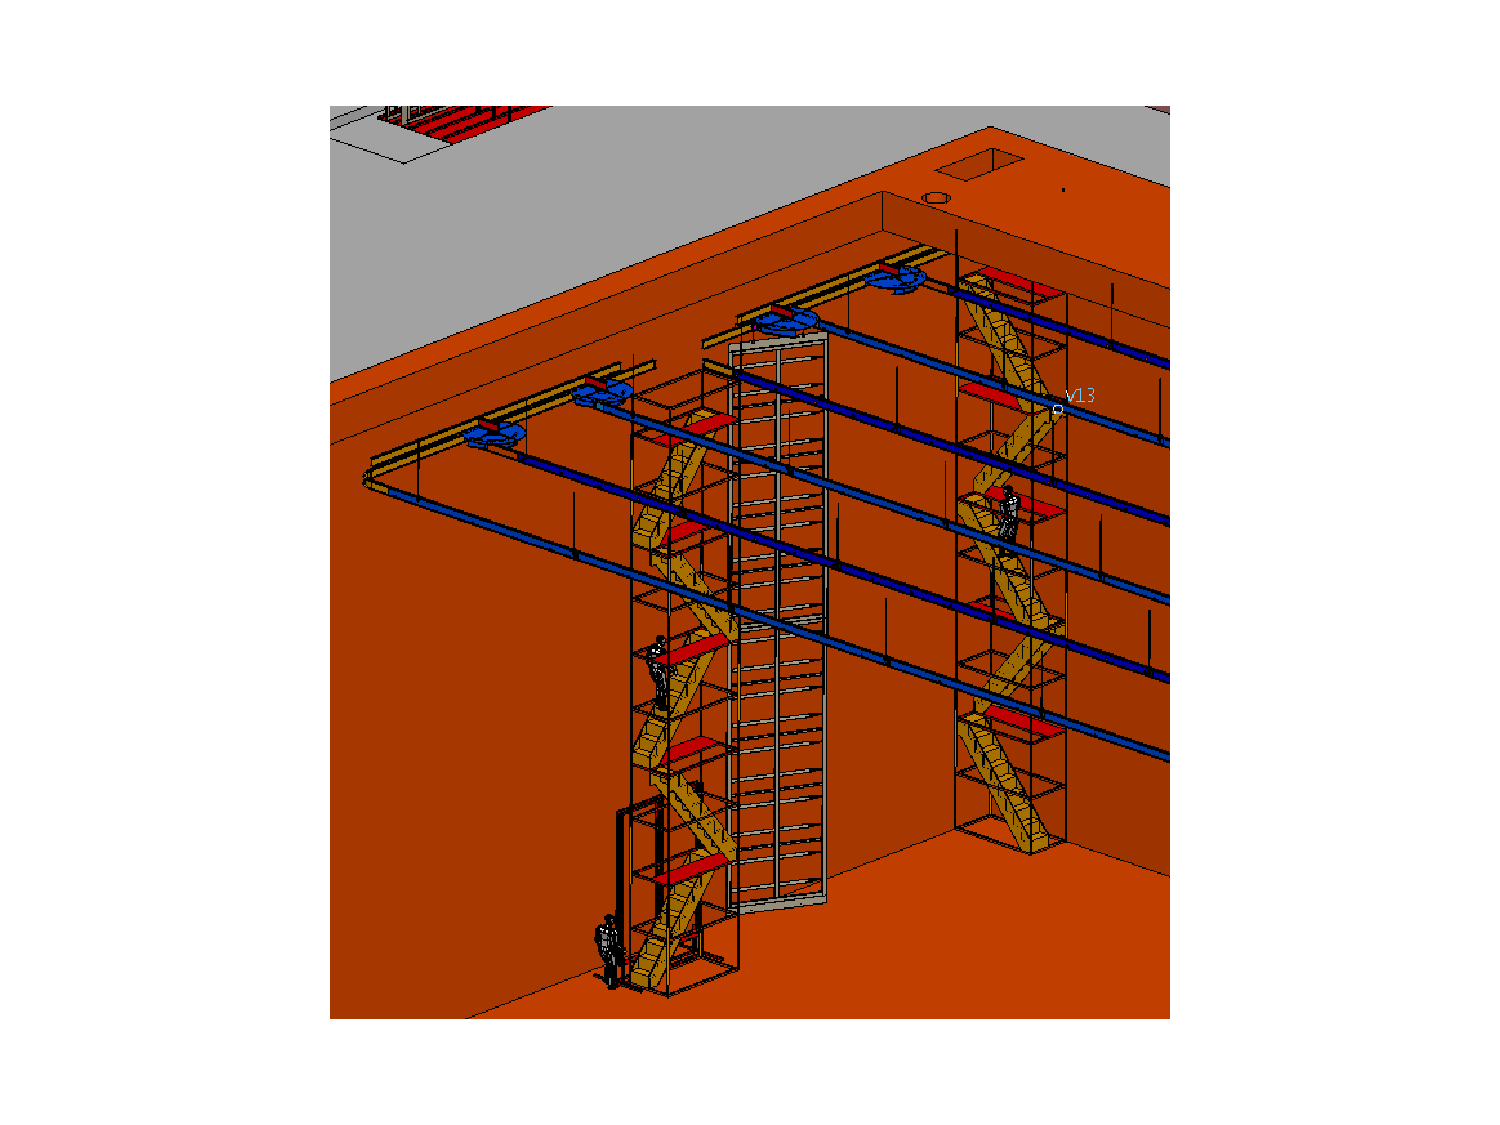
\includegraphics[width=\textwidth]{v5chIC_installation-monorail}
\caption{TPC installation monorail with APA moving to support rail}
\label{fig:installation-monorail}
\end{figure}

A rolling scaffold with an integral stair tower will allow personnel to access the top of the stacked panel. Fixed scaffolds with stair towers will provide access into the cryostat. 

\subsection{Detector Electrical Ground}

The LAr-FD will have nearly a quarter million channels of electronics with an intrinsic noise level of less than 1,000 electrons.  These channels will be connected to wires that are seven meters long.  Thus, grounding, shielding and power distribution are critical to the success of the experiment. In the reference design the entire cavern will be treated as the detector ground for the following reasons.

The cryostat has a large number of penetrations for supporting the APAs that extend to the support structure above the cryostat.   There are also 13 signal feedthrough ports which connect to racks located on the top of the cryostat.  Achieving and maintaining adequate AC isolation on such a large structure during construction will be difficult.  In addition, the cavern has very few connections to the outside world so it is much easier to isolate the cavern as  a whole than the individual pieces.

Secondly, it is necessary to provide a conductive body with a large enough self-capacitance that its voltage changes only negligibly when electric charge flows onto it. In this way the cavern can serve as a sink of unwanted current without generating noise in the detector.   

\subsubsection{Reference Design}

Earth ground will be provided by the Ufer grounding system in the concrete walls and other concrete support structures.   This ground will be attached to the rock bolts in the cavern walls and augmented by the large amount of steel in the roof-support trusses and the upper metal floor.  To be an effective ground, all of the steel support structure will be welded together.  The welds need not be structural; their use is only to assure reliable long-term electrical connections.

In order for this system to work, the cavern must be kept noise-free, i.e.,  all  connections, except AC power, between the cavern and the outside world must be electrically isolated either by dielectric breaks or optical isolators.  
Electric motors will be restricted to three-phase induction motors except for special, well-controlled cases.  Electric heaters will be controlled by switches rather than SCRs.  Digital equipment such as network switches will 
be run at frequencies of 30 MHz or higher whenever possible so that the noise remains outside the bandwidth of the TPC preamplifier.  Some equipment, such as switching power supplies, will still need special attention to ensure that they do not generate noise in the detector.  

As the only conducting link to the outside world, the AC power must be filtered to eliminate any electrical noise.  Since the currents are large, it is most economical to implement a filter using the inductance of the power cable itself along with some capacitors to form a capacitor-inductor filter.  


The reference design will keep the power for the conventional facilities and for each cryostat  independent of one another so that they can be operated independently. As shown in Figure~\ref{fig:Saturable_inductor} (top), one 500-KVA transformer for each cryostat along with a one-MVA transformer for the conventional facilities will be placed in a separate utility room located a short distance from the detector cavern. These transformers will have double faraday shielding with the primary shield returned on the ground wire to the substation.  The second shield will be connected to the local Ufer ground and to the cavern by the required grounding wire.  

A saturable inductor between the two shields serves to isolate the primary and secondary shields and separate their grounds.  The secondary shield and transformer frame are connected to Earth ground at the transformer.  The ground wire running back to the substation is only locally grounded through the saturable inductor but it is fully grounded at the substation.  A fault between the secondary and primary shields would trip the substation breaker due to current flowing in the return ground wire.  If this wire were disconnected, the current would flow through the saturable inductor to Earth ground and also trip the substation breaker.  Figure~\ref{fig:Saturable_inductor} (bottom) shows an inductor used at D-Zero and the voltage developed across the inductor as a function of the fault current.  The inductance is completely saturated by 100~A and the developed voltage is still safe.


The 480-V power will be transmitted from the utility room to a separate switch gear for each detector module. The switch gear, located adjacent to its module, will directly distribute power to all the 480-V loads. The switch gear will also feed up to three 50-KVA single-faraday-shielded transformers.  Two of these will provide 208-V power to the module and its associated cryogenic equipment, and the third will provide additional cavern power.  The number and size of the transformers may change depending on the final load. 

The filter on the conventional-facilities transformer will be similar to the one for the detector modules.  In addition to the conventional facilities, this transformer will power all welding outlets.  This arrangement would allow some minor welding on one cryostat, if needed, while the other is taking data. 

\begin{figure}[htpb]
\centering
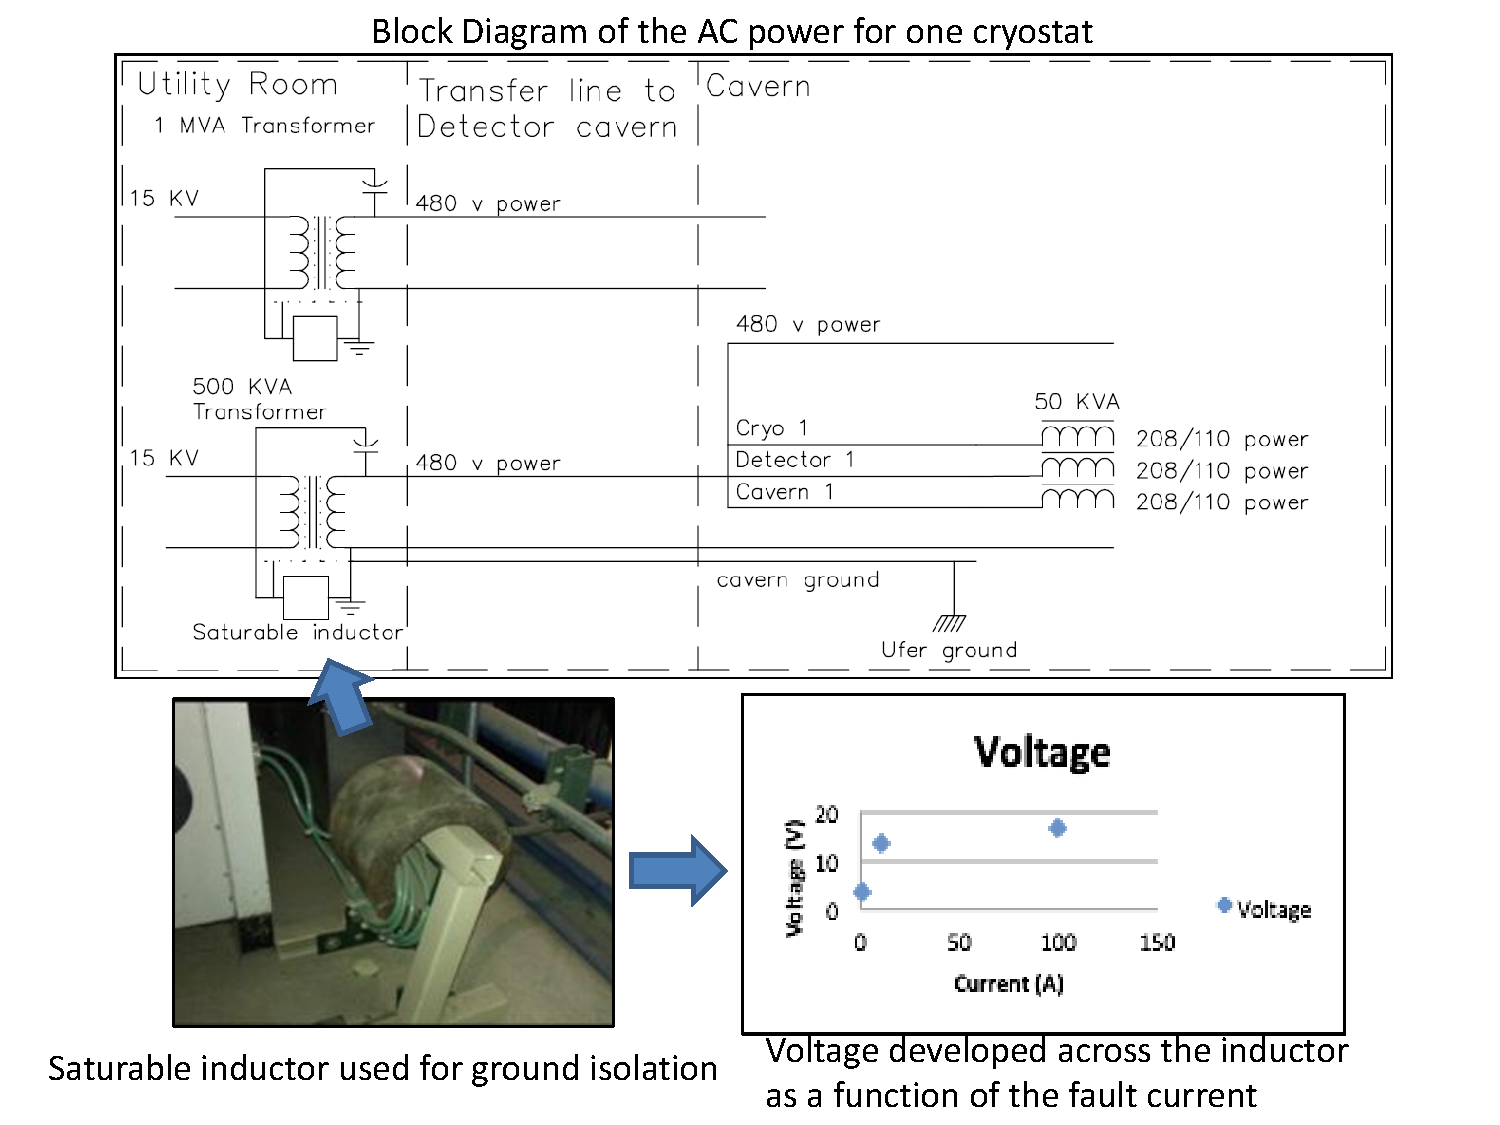
\includegraphics[width=\textwidth]{v5chIC_Marvins_saturable_inductor}
\caption[Block diagram of the AC power for one cryostat]{Block diagram of the AC power for one cryostat with a saturable inductor to separate the grounds of the transformer shields}
\label{fig:Saturable_inductor}
\end{figure}

\subsubsection{Features}

%Internal Detector Ground Connection:  
It is important that all the components inside each detector module be connected to a common ground.  The  best candidate for this common ground, and the one chosen for the reference design, is the top of the cryostat.  The APAs will have ground braid connections to the roof at two points on each panel.  The lower APAs will be connected to the upper ones by their mechanical mounting connections.  The front-end boards, phototube ground and the reference ground for the bias voltages will all be connected to the APA frame.

%Detector ground plane: 
The top of each cryostat is made of 1.2-mm or 2.0-mm-thick stainless steel, a poor conductor, and therefore does not serve as an adequate ground plane.  The best solution would be to add a copper sheet directly on top of the cryostat, however this is difficult to do. Instead the copper sheet will be installed over the insulation that is on top of the cryostat membrane, about one meter from the cryostat, and connected to it via a grid of connections spaced 2.5~m apart.  This spacing will give good electrical performance up to 12~MHz -- well above the input bandwidth of the amplifier. The connections will be made with copper strips that fit in gaps in the insulation. Power supplies and power-supply filters (including the cathode supply) will all be grounded to this plane.

%Cables and Racks: 
A port is located above every other APA junction and each port will serve the four APAs located directly underneath it.  Cables for the bottom two APAs will be routed through the hollow cable frames to provide both mechanical support and electrical shielding.  The digital cables will be located in the left frame member, and the power and bias lines will be routed through the right frame member.  The horizontal portion of the cable run will be outside of the wire planes, so the use of doubly shielded cable such as Amphenol skew clear 
%\fixme{the cable is called 'amphenol skew clear"? BB: Yes. Marvin is using it as an example of an existing commercially available cable. } 
may be adequate.   If  not, then custom metal shields will be mounted on the front-end circuit boards.

The racks will be mounted either directly over the ports or adjacent to them with an extension to the rack that covers the port. All cables can be brought out of the cryostat into a grounded and shielded enclosure.  %In order to have equal times to all APAs, 
All cables to the APAs will be the same electrical length to ensure uniformity of signal travel time.  This will require storing an extra 14 meters of cable for each top  APA.  The plan is to use 36-in-deep racks and construct a shielded area on the back side of the rack to hold the excess cable.  Twenty-seven racks will be required for each cryostat, and rack space will be shared between the TPC and photon-detection system readout and power supplies. A modest number of racks will be required for the DAQ in the surface control room. All relay racks will be equipped with rack protection and monitoring. The racks will be supplied by the detector installation effort.

%Digital Electronics: 
The digital electronics does not present a grounding issue in the strict sense, but it does affect noise.  The plan is to operate the digital system with at least a 32-MHz clock that is well above the upper bandwidth of the input amplifier (the 3-db point is less than 1~MHz).



%%%%%%%%%%%%%%%%%%%%%%%%%%%%%%%%%%%%%%%%%%%%%%

\section{Below-ground Installation Activities}

The following list of detector components and systems % are installed in this WBS element.  
will be installed below-ground:

\begin{itemize}
\item Relay Racks with rack protection (10 on each cryostat plus a few in the control room)
\item Cable trays and power distrbution to racks
\item Cable inside and outside of the cryostat including cable feedthroughs
\item DAQ crates and power supplies in the relay racks
\item The 52 APAs per cryostat with integrated photon detectors
\item The 78 CPAs per cryostat
\item Any cryogenic instrumentation not installed by the cryostat construction vendor (e.g. purity monitors)
\item Note: Support rails and hangers are installed during cryostat construction
\end{itemize}

\begin{figure}[htpb]
\centering
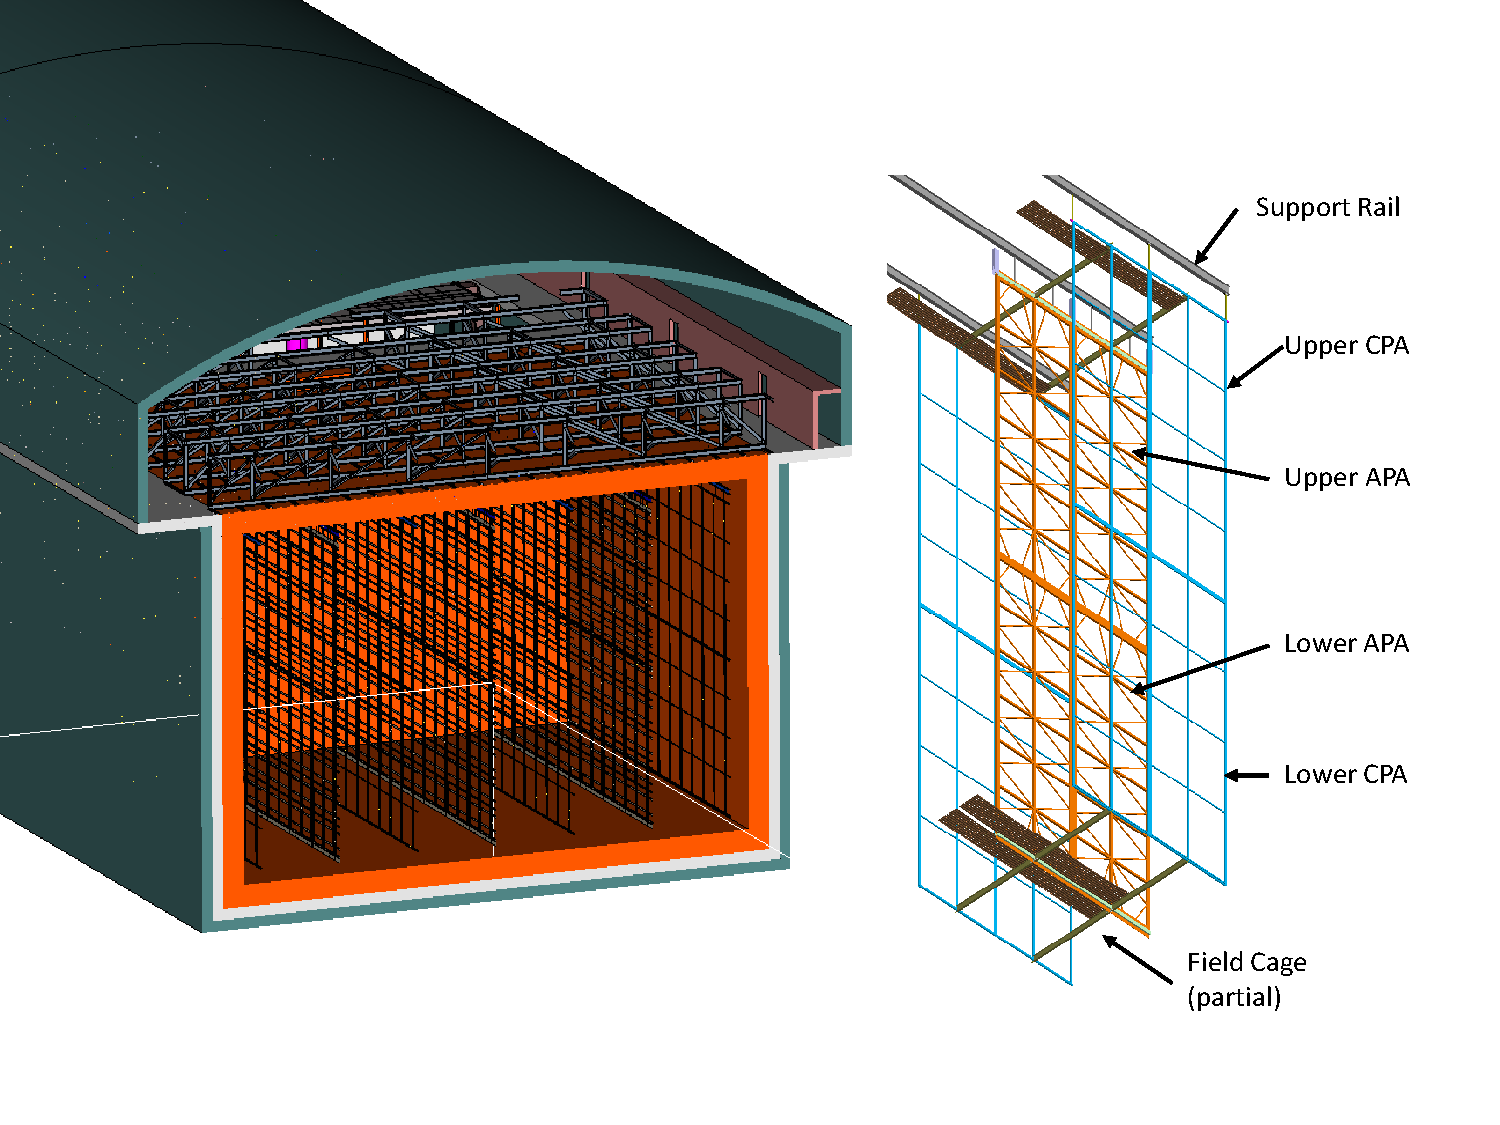
\includegraphics[width=\textwidth]{v5chIC_tpc-panels-installed-in-cryostat}
\caption{TPC panels installed in cryostat 
}
\label{fig:tpc-panels-installed}
\end{figure}

\section{TPC Installation}

Each APA and CPA panel will be carefully tested after transport into the clean area at the septum and before installation into one of the cryostats.  Immediately after a panel is installed it will be rechecked. Throughout the installation period it will be checked periodically. The serial stacking of the APA and CPA panels along the rails means that removing and replacing one of the early panels in the row after several others are installed would be very costly in effort and time. Therefore, to minimize the risk of damage,  as much work around already-installed panels as possible will be completed before proceeding with further panels.

The installation sequence is planned to proceed as follows:

\begin{enumerate}
\item Install the monorail or crane in the staging area outside the cryostat, near the equipment hatch.
\item Install the relay racks on the top of the cryostat and load with the DAQ and power-supply crates.
\item Dress cables from the DAQ on the top of the cryostat to remote racks.
\item Construct the clean-room vestibule outside the cryostat hatch.
\item Install the raised-panel floor inside the cryostat.
\item Insert and assemble the stair tower and mobile scaffold.  
\item Install the transfer rail with switches and the staging platform inside the cryostat
\item Install protection on (or remove) existing cryogenics instrumentation in the cryostat.
\item Install the cryostat feedthroughs and dress cables inside the cryostat along the support beams.
\item Begin regular transport of TPC panels in shipping boxes into the cavern.
\item Install TPC panels
panels:
\begin{enumerate}
\item Install a connected APA-CPA panel pair.
\item Connect power and signal cables.
\item Test each APA wire for expected electronics noise. Spot-check electronics noise while cryogenics equipment is operating.
\item Connect field cage in sections as the APA and CPA installation progresses.
\item Perform electrical test on CPAs and field cage.
\item Remove temporary floor sections as the TPC installation progresses.
\item Install sections of argon-distribution piping as the TPC installation progresses.
\end{enumerate}
\item Complete the field cage.
\item Remove the transfer rail, staging platform, moving platform and stair tower.
\item Temporarily seal the cryostat and test all channels for expected electronics noise.
\item Seal the access hatch.
\item Perform final test of all channels for expected electronics noise.
\end{enumerate}

In general, APA and CPA panels will be installed in order starting with the panel furthest from the hatch side of the cryostat and progressing back towards the hatch. The field cage will be installed in stages as the installation of APA and CPA panels progresses. The only requirement for survey or alignment is to maintain the edges of a row of APA panels to 3-mm alignment along each beam. A laser guide or optical transit in combination with the adjustment features of the tie rods will be used to establish the alignment. After the stacked panel is attached to the support rods the electrical connections will be made to cables that were already dressed to the support beams and electrical testing will begin. Periodic electrical testing will continue to assure that nothing gets damaged during the additional work around the installed panel. 

The TPC installation will be performed in three stages, each in a separate location; the locations, or zones, are shown in Figure~\ref{fig:work-zones}. 
First, in the clean room vestibule, a crew will move the APA and CPA panels from storage racks, rotate to the vertical position and move them into the cryostat. 
Secondly, in the panel-staging area immediately below the equipment hatch of the cryostat, a second crew will transfer the lower panels from the crane to the staging  platform, connect the upper and lower panels together, route cables to the top of stacked panels and finally transfer the stacked panels on to the monorail trolley that moves within the cryostat. 
A third crew will reposition the movable scaffolding and use the scaffold to make the mechanical and electrical connections at the top for each APA and CPA as they are moved into position. The  monorails inside and outside the cryostat will each have two motorized trolleys so that work can be conducted by all three crews in parallel. 
The steady-state rate for installation, given this work plan and a single-shift schedule, is estimated to be two stacked panels per day. 

\begin{figure}[htbp]
\centering
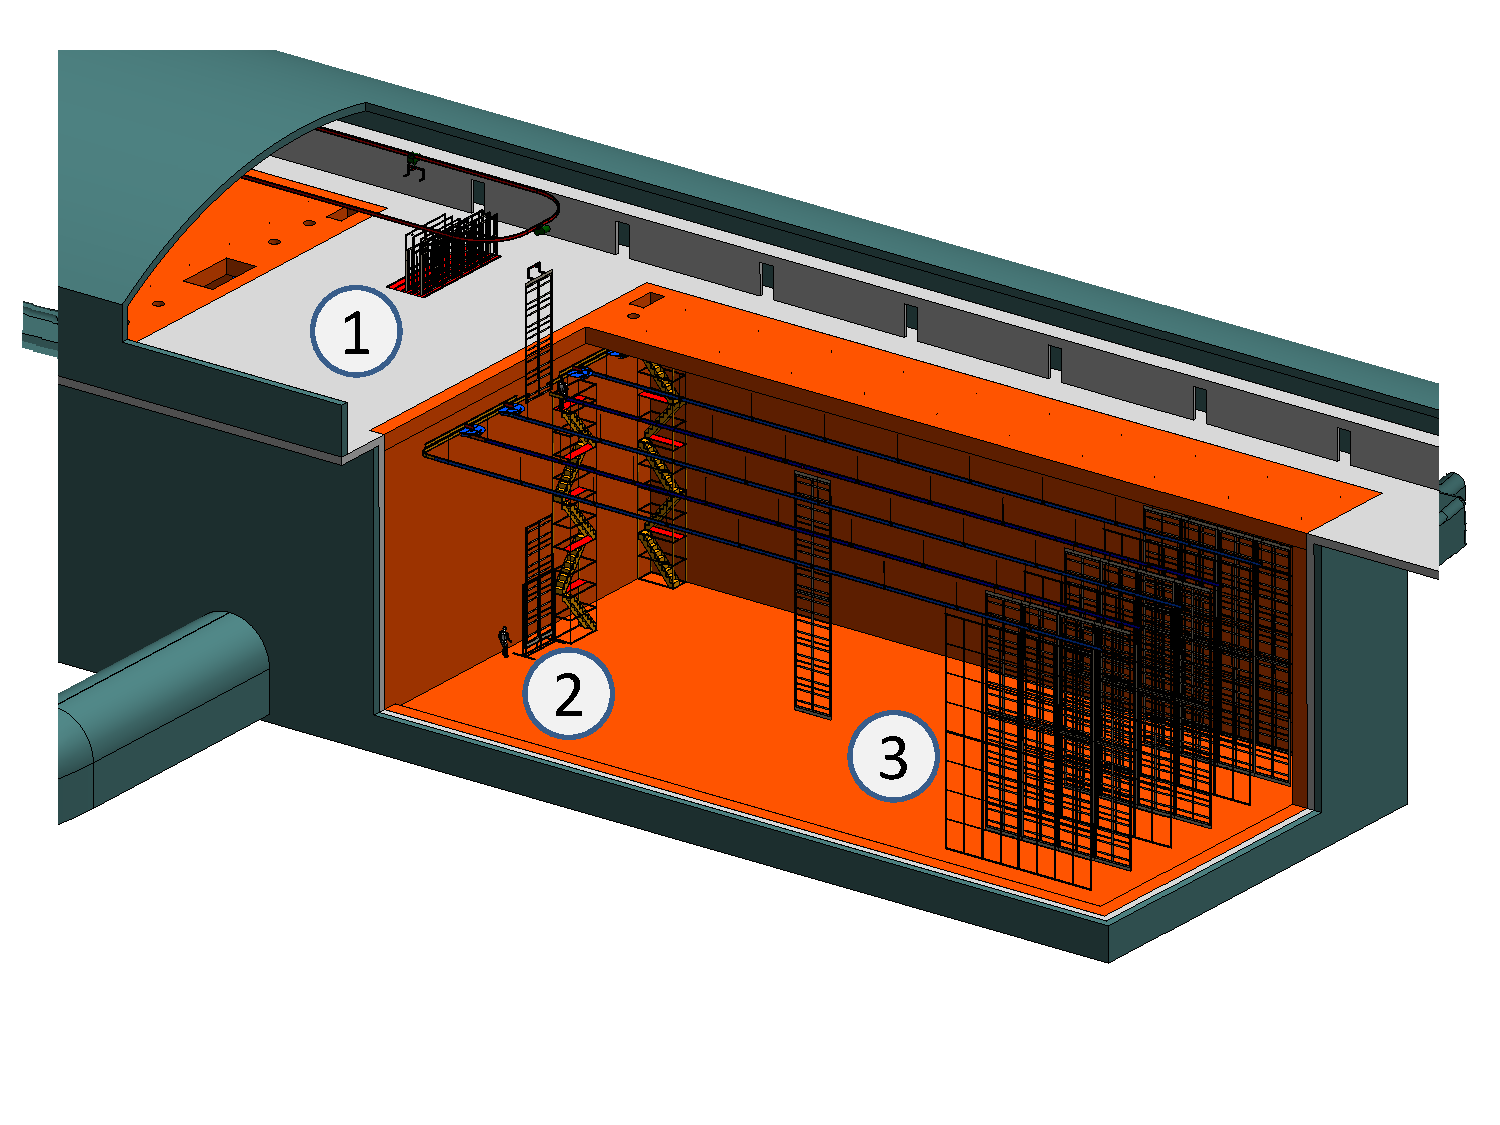
\includegraphics[width=\textwidth]{v5chIC_work-zones}
\caption[The three main work zones for TPC Installation]{The three main work zones for TPC Installation. TPC components are lowered into the cryostat in zone 1. TPC components are connected together in zone 2, transferred to the support rails and then rolled into final position (zone 3).}
\label{fig:work-zones}
\end{figure}

Wire integrity will be confirmed by measuring the Equivalent Noise Charge (ENC) of each electronics channel and comparing it with the expected noise for a properly connected wire. A properly connected wire provides an input capacitance of 240~pF to the front-end amplifier resulting in an ENC at room temperature of 1,100 electrons.
The wire-integrity test also ensures that coherent noise sources, e.g., a mechanical connection between the detector ground and the Ufer ground, are discovered promptly. Error budgeting, regular noise monitoring and mitigation will ensure that the TPC reaches and maintains the required noise performance before the cryostat is cooled down.


The detector installation system is also responsible for developing and implementing the procedure for monitoring the integrity of the membrane-cryostat primary liner during installation.  The space between the primary liner and the secondary liner will be held under vacuum during installation. The vacuum level will be automatically monitored and will alarm if any leaks develop in the primary membrane during TPC installation.

%%%%%%%%%%%%%%%%%%%%%%%%%%%%%%%%%%%%%%%%%%%%%%

\section{Installation Prototype} 

The goals of the installation prototype are to test and verify the key elements of the equipment and process for TPC installation and to serve as a training tool for personnel who will perform the TPC installation. The initial testing of the equipment at Fermilab will be used to verify or refine the installation concepts. Complete testing of the final equipment and operations will occur at Fermilab before the installation equipment is moved to the Far Site. 

For the installation prototyope, a similar, 70\%-height detector will be constructed in a suitable location at Fermilab, e.g. the Wideband lab or the CDF or DZero assembly hall. 
The cryostat mock-up will include a representation of a roof hatch, APA and CPA rail supports and feedthroughs. 
Multiple mock-ups of APA and CPA stacked panels will be installed. The APAs will include all mechanical mounting points and electrical connections such as optical-fiber readout cables and power cables.
Prototype versions of the special equipment required for TPC installation will be used, including the lower panel staging platform, a transfer rail with trolley, and rolling-cart scaffolding. Scaffolding elements will be rented and the scaffolding will be erected by a contract or as part of a training program.

Initial tests, where appropriate, will be peformed at a low elevation. For example, the installation trolley and single-switch rail segment will be tested at a low elevation with a dummy weight. After successful demonstration of the features  at low elevation, the components will be moved to a high elevation for testing with full size mock-up panels.



%%%%%%%%%%%%%%%%%%%%%%%%%%%%%%%%%%%%%%%%%%%%%%

\section{Training and Access Control}

Installation and Commissioning will be responsible for the personnel, equipment and procedures for providing cavern-access controls. These controls will include a mechanism for checking the training status of personnel, badge-in/badge-out procedures and closed-circuit-television monitoring of the entrance portal. Only trained personnel will be allowed below-ground. Members of the installation crew will be trained on specific installation tasks and must pass a qualification test. The training will likely use mock-up APAs constructed for the installation prototype. The training program will be modeled after the Fermilab ``NuMI underground training'' and will be developed in collaboration with Sanford Laboratory ES\&H personnel.

Installation and Commissioning will provide all of the general tools and equipment needed to support the personnel in their installation work. It will include hand tools, power tools, material-handling equipment, ladders, lifts, electrical meters and personal protective equipment (PPE). The detector sytem groups will provide any special equipment to check out or debug the power and read-out chain of the detectors.

%%%%%%%%%%%%%%%%%%%%%%%%%%%%%%%%%%%%%%%%%%%%%%

\section{Detector Commissioning}

The construction  of the two cryostats and the installation and commissioning activities will be staged such that both TPCs can be tested cold while one cryostat still remains available as a potential storage vessel. The LAr in one cryostat can be transferred to the other, and back again, if necessary. Once both TPCs are known to work properly at LAr temperature, the second fill will take place.

The commissioning sequence, illustrated in Figure~\ref{fig:startup_sequence}, will start with the installation of the TPC in the east cryostat. During this time, construction of the west cryostat will be 
completed.  The east cryostat will be filled initially with room-temperature GAr, injected from the bottom 
in order to displace the air upward through the top ports. The procedure used for this gas purge will be developed during prototype work. Following that, the LAr fill of the east cryostat will take four to six months, 
assuming continuous LAr deliveries.  LAr purification will begin when the liquid level is high enough to start the recirculation pumps. The commissioning of the cryogenics system can also begin at this point but its full commissioning will require a fully loaded cryostat. When the cryostat is full, the TPC will undergo testing for about one month. In-vessel purity monitors will operate during this time.

\begin{figure}[htpb]
\centering
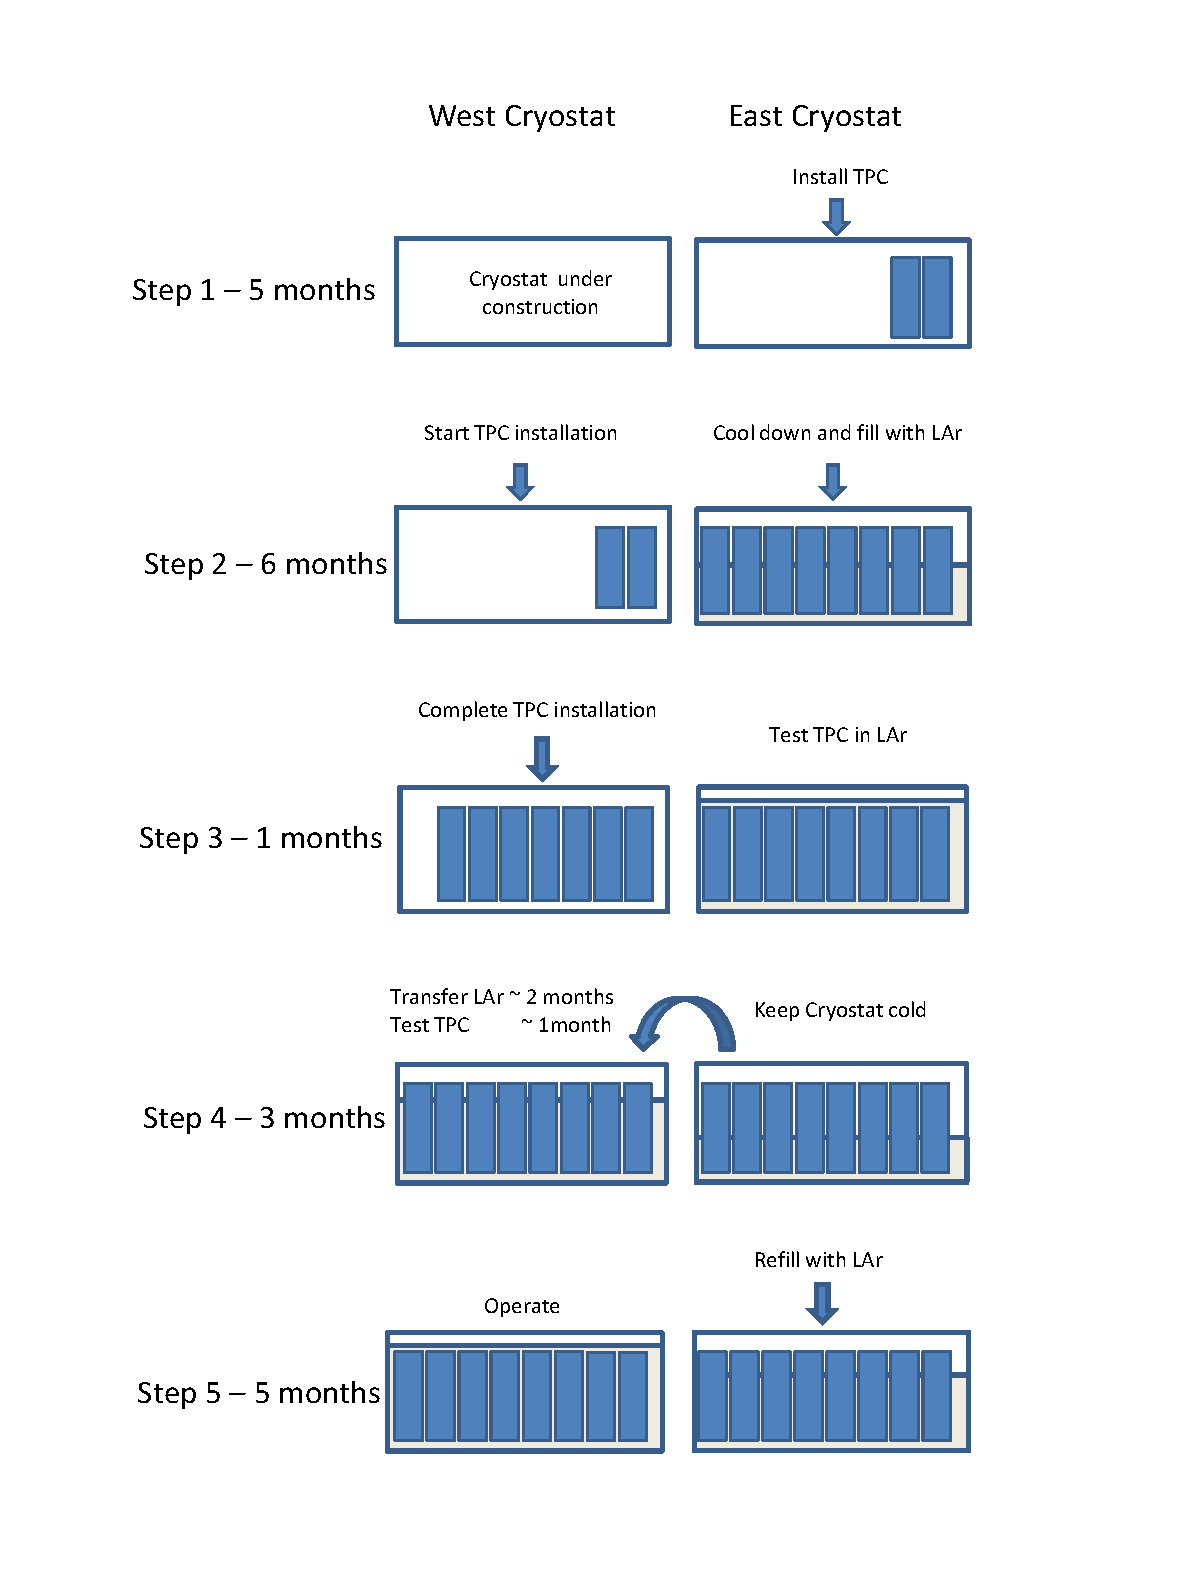
\includegraphics[width=\textwidth]{v5chIC_startup_sequence}
\caption{Startup and Commissioning Sequence}
\label{fig:startup_sequence}
\end{figure}

Construction of the west cryostat is expected to finish during the LAr fill of the east cryostat. After the west cryostat is leak-checked and cleaned, its TPC installation will begin. After TPC installation and testing, the purging and cooling phases will proceed. Then the LAr from the east cryostat will be transferred to the west one, at which point the west TPC will begin a month of testing. During this time the east cryostat will be maintained cold via continuous GAr circulation. Once tests on the west cryostat are completed successfully, the east cryostat will be refilled with LAr, and its roughly five-month commissioning period begins. 

\section{ES\&H}

Careful consideration for ES\&H will be demonstrated in the planning and execution of the installation and commissioning. Safety professionals will be involved in all phases. Hazards of note for the TPC installation are work at elevated heights and working in the confined space of the cryostat. 

